\subsection{参数方法}
\subsubsection{什么是曲面}
曲面是空间中非常有规律(regular enough)的一组点。空间中点的随机分散不符合我们对曲面的直观概念。例如,它不够规律。另一方面,球面的边界确实符合我们对曲面的概念,也就是说,由于球面是“光滑的”,所以它具有足够的规律来作为曲面。
\begin{figure}[H]
\centering
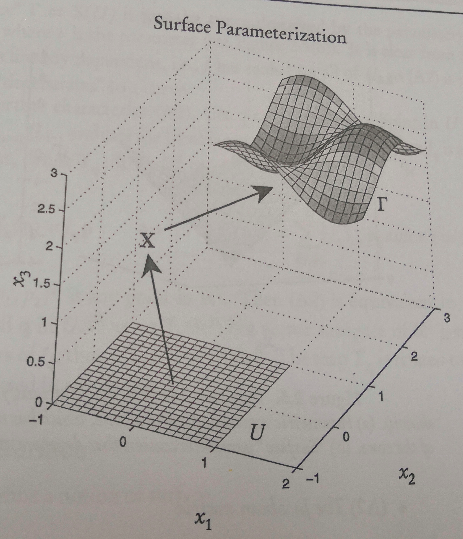
\includegraphics[scale=0.5]{./figures/24.png}
\caption{参数表示的例子。参考域$U$是$x_1,x_2$平面上的方形显示。映射$X$将集合$U$对应于曲面$\Gamma$(曲面基于$x_3$坐标着色)。}
\end{figure}

直观地说,我们可以把创建一个表面想象成把一个平的橡胶板变形成一个弯曲的板。第$2.1.6$节中的变换$X$捕捉到了这个思想。因此,令$U \subset \mathbb{R}^2$是一个“平”域,令$X$:$U\Rightarrow \mathbb{R}^3$是个变形变换,例如,对于$U$中的每一个点$(s_1,s_2)^T$都对应于$\mathbb{R}^3$的点$x= (x_1,x_2, x_3)^T$使得
\begin{gather}
\mathbf{x}=X(s_1,s_2).
\end{gather}
令$\Gamma=X(U)$表示由“变形”$U$得到的曲面。我们称$(2.10)$是曲面$\Gamma$的参数表示,其中$s_1,s_2$称为表达参数。有时,我们把$U$作为一个参考域。有关$(2.10)$的示例,请参见图$2.4$。\\
\textbf{允许参数化}\\
如果我们要用$(2.10)$来定义曲面,那么我们必须对$X$进行假设,以保证$\Gamma=X(U)$是一个有效的曲面。最起码,X必须是连续的,以避免“撕裂”橡胶板。但是如果我们想对$\Gamma$做微积分,我们实际上需要更多。\\
\textbf{假设1.}我们对$X$做如下规律性假设。\\
$\bullet$ $(A1)$函数$X(x_1,x_2)$在$U$上是$C^{\infty}$,$\Gamma$中的每个点$\mathbf{x} = X(s_1,s_2)$对应于$U$中的一个点$(s_1, s_2)$,$X$是单射。
\begin{figure}[H]
\centering
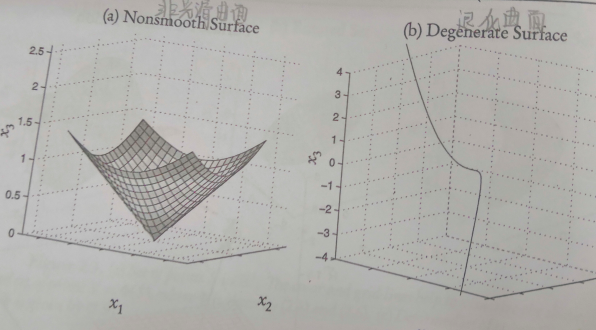
\includegraphics[scale=0.5]{./figures/25.png}
\caption{这里的例子不满足假设$1$(参考域$U$没有显示)。$(a)$是一个圆锥体的参数表达,它在圆锥体的角上不能定义切平面。$(b)$是一个曲线,退化的曲面}
\end{figure}
$\bullet~(A2)$雅克比行列式(Jacobian)在$U$上秩为$2$,$J$ 的列向量是线性无关的。
\begin{gather}
J=\left[ \partial _{s_1}X,\partial _{s_2}X \right]=
\begin{bmatrix}
\partial _{s_1}X_1  & \partial _{s_2}X_1 \\
\partial _{s_1}X_2  & \partial _{s_2}X_2 \\
\partial _{s_1}X_3  & \partial _{s_2}X_3 
\end{bmatrix}
\end{gather}

我们说方程$(2.10)$的参数满足$(A1)$和$(A2)$是参数化的,用更现代的话说,immersion
\textbf{重要性}\\
假设$(A1)$对平面施加了一定的光滑性,即在$\Gamma$中的每一点上都有定义良好的切平面。切平面的精确定义见第$2.4.3$节;现在,我们只需要一个切平面的直观概念。例如,令$U=(-1,1)\times (-1,1)$并且考虑映射
\begin{gather}
X(s_1,s_2)=(s_1,s_2,\sqrt{s_1^2+s_2^2})^T~~~~~~~~(s_1,s_2)^T\in U.
\end{gather}
曲面$\Gamma = X(U)$是一个圆锥(见图$2.5(a)$)。很明显,$(2.12)$在$(0,0)^T$处不可导,即$(A1)$是无效的。因此,不存在唯一通过$(0,0,0)^T$且与表面$\Gamma$“相切”的平面。

需要假设$(A2)$来避免集合$\Gamma$(由$(2.10)$参数化)为$\mathbb{R}^3$中的曲线的可能性。通过线性代数,$A(2)$等价于$\partial _{s_1}X \times \partial _{s_2}X\neq 0$,这也等价于在$\mathbb{R}^3$中$\partial _{s_1}X$和$\partial _{s_2}X$是线性无关的向量。例如,令$U= (-1,1) \times (-1,1)$并且考虑映射
\begin{gather}
X(s_1,s_2)=(s_1+s_2,(s_1+s_2)^2,(s_1+s_2)^3)^T~~~~~~~~(s_1,s_2)^T\in U.
\end{gather}
“曲面”$\Gamma =X(U)$就是通过$X(t)=(t,t^2,t^3)^T$参数化后的曲线,其中t为参数(见图$2.5(b)$)。由$(2.13)$可知,$\partial _{s_1}X$和$\partial _{s_2}X$是线性相关的,即,在所有$U$上秩都是1,所以$(A2)$ 无效。因此,表面“退化”成曲线。

我们进一步描述$(A2)$。令$\mathbf{q}=(q_1,q_2)^T$为$U$中的一个点,定义$J^{q}=\left[ \partial _{s_1}X,\partial _{s_2}X \right]|_{s=q}$,(求出该点的雅可比矩阵)。注意$J_p$是$\mathbb{R}^{3\times 2}$中的一个常数矩阵。接下来,定义$T_q:\mathbb{R}^2 \Rightarrow \mathbb{R}^3$
\begin{gather}
T_q(\mathbf{p})=J_q \mathbf{p}~~~~~~~\Leftrightarrow~~~~~~~(T_q(\mathbf{p}))_i=\sum_{k=1}^{2}(J_q)_{ik}p_k~~~i=1,2,3,
\end{gather}
其中$\mathbf{p}= (p_1,p_2)$是$\mathbb{R}^2$中的任意一点。那么$(A2)$等价与映射$T_q$,是$U$中所有$\mathbf{q}$单射。集合$T_q(\mathbb{R})^2$是$J_q$中两个列向量产生;因此,它的维数是$2$。映射$T_q$与切平面有关,这将在$2.4.3$节中讨论。

\subsubsection{曲面参数化}
现在我们可以定义曲面的概念。

\textbf{定义1(参数曲面)}。令$U \subset \mathbb{R}^2$是一个开集并且考虑一个映射$X:\Rightarrow \mathbb{R}^3$。如果$X$在$U$中是可微的,我们称$(U,X)$是一个参数曲面。如果映射$T_q$对于所有$U$中的$\mathbf{q}$是单射,则称$X$是正则的(regular)。此外,如果有一个$U$中的$\mathbf{p}$不是单射,或未定义,则我们称$\mathbf{p}$时$X$的一个奇异点;否则,这是一个正则点。\\

注意,我们将这对$(U,X)$称为参数曲面,因为$\Gamma=X(U)$是构成曲面的点集,$U$和$X$描述了如何在$\Gamma$上“绘制”坐标曲线。进一步阐述可以见图$(2.4)$。参考域$U$只是组成一个正方形的一组点。然而,$U$上的网格线对应于$U$上的坐标系统,这些网格线通过$X$映射到$\Gamma$(见图$2.4$),这定义了$\Gamma$上的一种曲线坐标系。

如果我们在$U$上选择了一个不同的坐标系,那么网格线在$U$(和$\Gamma$)上看起来就会不一样。在$\Gamma$上会有一个不同的曲线坐标系(参见图$2.10$)。

因此,曲面可以以多种方式参数化就不足为奇了。实际上,给定$\Gamma$的一个参数化$(U,X)$
\begin{gather}
s_1=s_1(\tilde{s}_1,\tilde{s}_2),~~~s_2=s_2(\tilde{s}_1,\tilde{s}_2),~~~(\tilde{s}_1,\tilde{s}_2)^T \in ~\tilde{U}
\end{gather}
即,$s:\tilde{U} \rightarrow \mathbb{R}^2$和$U=s(\tilde{U})$。接下来,定义$\tilde{X}=X\circ s$,意味着
$$\tilde{X}(\tilde{s}_1,\tilde{s}_2)=X(s_1(\tilde{s}_1,\tilde{s}_2),s_2(\tilde{s}_1,\tilde{s}_2)).$$
这里$(\tilde{U},\tilde{X})$也是$\Gamma$的一个参数化。可以把$s$当成$\tilde{U}$到$U$的映射($s^{-1}$看成$U$到$\tilde{U}$的映射)
\begin{figure}[H]
\centering
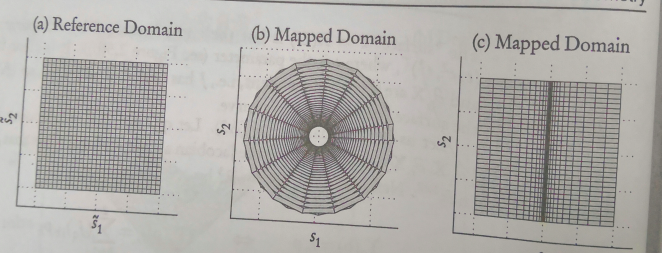
\includegraphics[scale=0.5]{./figures/26.png}
\caption{所示图是不满假设$2$的例子。$(a)$是参考域。$(b)$是使用$(2.17)$中的映射$U$映射到一个环,注意这个环面覆盖了两次。$(c)$是使用$(2.18)$中的映射$U$映射到一个方形。网格线在$s_1$的附近挤压在一起}
\end{figure}

当然,为了有一个正则的参数化,我们必须有假设$1$必须满足$(\tilde{U},\tilde{X})$。这需要对$(2.15)$做以下假设。\\
\textbf{假设2.}\\
$\bullet~(A0*)$方程$(2.15)$被定义在区域$\tilde{U}$上且使得$U=s(\tilde{U})$。\\
$\bullet~(A1*)$方程$(2.15)$在$\tilde{U}$上是$C^{\infty}$,并且它是单射的。\\
$\bullet~(A2*)$雅克比矩阵
\begin{gather}
D=\left[ \partial _{\tilde{s}_1}s,\partial _{\tilde{s}_2}s \right]=
\begin{bmatrix}
\partial _{\tilde{s}_1}s_1  & \partial _{\tilde{s}_1}X_1 \\
\partial _{\tilde{s}_1}s_2  & \partial _{\tilde{s}_2}X_2 
\end{bmatrix}
\end{gather}
对于$\tilde{U}$上所有点$(\tilde{s}_1,\tilde{s}_2)$是非奇异的,即在$\tilde{U}$上$det(D)\neq 0$

我们说形如满足假设$2$的$(2.15)$的变换是一个允许的坐标变换(allowable)。

条件$(A1*)$和$(A2*)$彼此完全独立,实际上
\begin{gather}
s_1=e^{\tilde{s}_1}\cos (2\pi \tilde{s}_2),~~~~~s_2=e^{\tilde{s}_1}\sin (2\pi \tilde{s}_2)
\end{gather}
当$-1 \leq \tilde{s}_2 \leq 1$时是非单射的变换;然而,一个简单的计算给出$det(D) = (2\pi)^2e^{2\tilde{s}_2}$,它在$s_1,s_2$平面上从不为零(参见图$2.6$)。另一方面,变换
\begin{gather}
s_1=\tilde{s}^3 ,s_2=\tilde{s}
\end{gather}
处处都是单射,但是一个简单的计算得到$det(D)=3\tilde{s}_1^2=3\tilde{s}_1^{2/3}$,当$s=0$时,在整个$s_2$轴上它为零。(见图$2.6$)

